\documentclass[12pt,b6book]{book}

\usepackage{xltxtra}
\setmainfont[Ligatures=TeX]{IPAPMincho}
\setsansfont{IPAPGothic}
\setmonofont{IPAGothic}
\XeTeXlinebreaklocale "ja"
\usepackage{graphicx}
%\usepackage[unicode]{hyperref}
\usepackage{hyperref}
\usepackage{pdfpages}

\usepackage{listings}
\lstset{%
  backgroundcolor={\color[gray]{.85}},%
  basicstyle={\small},%
  frame={tb},
  breaklines=true,
  columns=[l]{fullflexible},%
%  lineskip=-0.5ex%
}
\usepackage{verbatim}

\usepackage{ulem}

% myjapanese.sty
\RequirePackage{xltxtra}
\def\en#1{{\engrm#1}} % 欧文フォントで出力
% 日本語を含む段落を行分割するための設定
\XeTeXlinebreaklocale ``ja''
\XeTeXlinebreakskip=0pt plus 1pt minus 0.1pt
\XeTeXlinebreakpenalty=0
% 半角分戻る
\def\<{\@ifstar{\zx@hwback\nobreak}{\zx@hwback\relax}}
\def\zx@hwback#1{\leavevmode#1\hskip-.5em\relax}
% 簡易レイアウト設定
\RequirePackage[scale=0.8, margin=1in]{geometry}
%\RequirePackage{indentfirst}
\RequirePackage{setspace}
\setstretch{1}
\parindent=1em

\begin{document}

\frontmatter
%% 表紙
%% \pagenumbering{Alph}
%%\insertpage{images/KOKORO100.pdf}
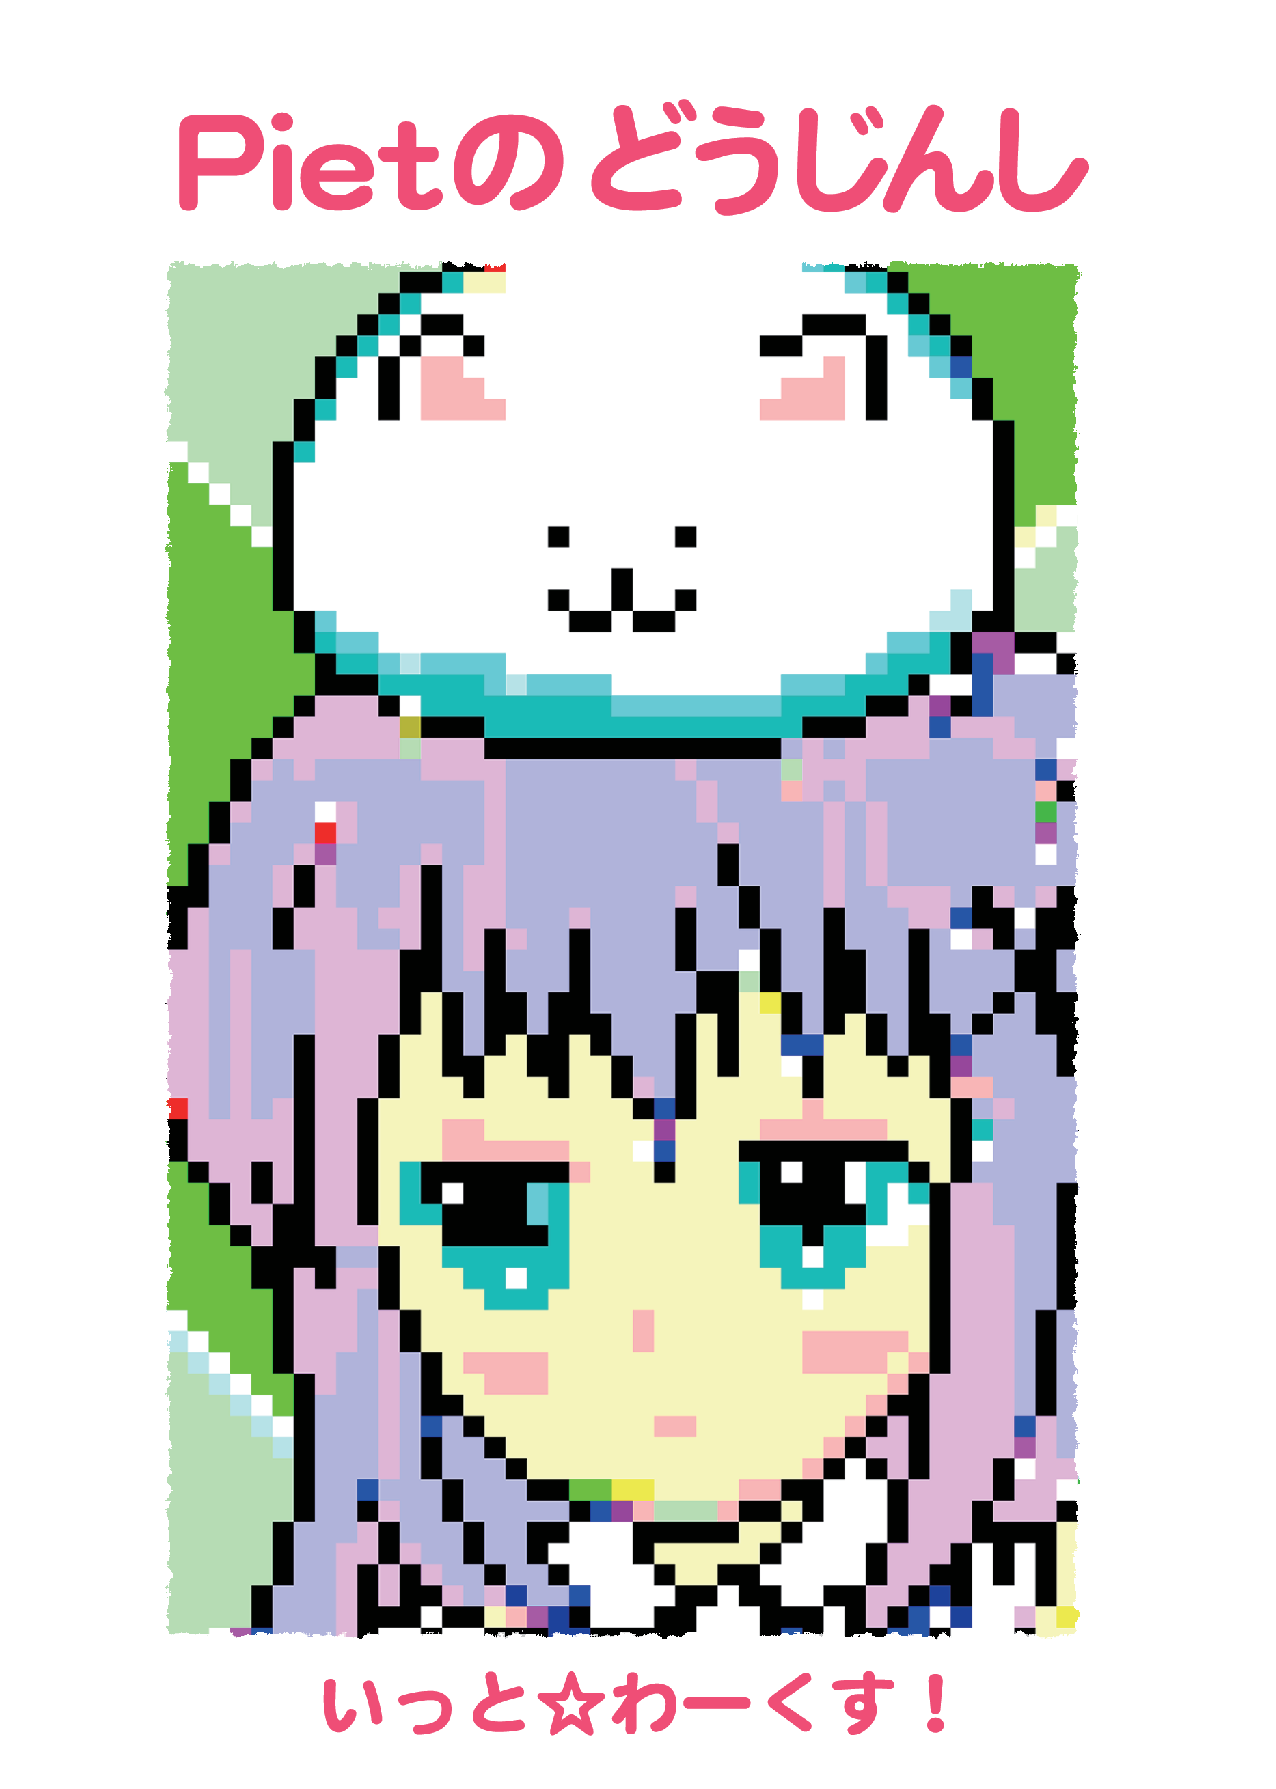
\includepdf{images/hyoushi.pdf}
%%
\includegraphics[width=\paperwidth]{images/KOKORO100.png}
%% \addtocounter{ptc}{1} % nande-
\tableofcontents
%% \newpage
%%  
%% \newpage

\mainmatter

\chapter[Pietの自動生成]{Pietの自動生成}

\section{はじめに}

こんにちは、NoNameA 774です。
KMC(京大マイコンクラブ)というPietサークルに入っているのですが、
サークルの人々がPietを手で(書いてる\textbar{}描いてる)のを見て、
絵としての意味を持つ方法以外でPietを人間が描くのは不毛だと思い、
Pietの自動生成を行いたいと思った次第です。
今回一度ぐらいサークル参加をしてみたいとコミケに初申し込みしてみたら、
運良く当選したのでこの本を書いている次第です。

前回のコミケ(C88)でも同じようなペーパーを出したので(\url{https://nna774.net/piet/})、
それの\sout{焼き直し}続きのような感じです。
前回のペーパーは二日目のアース・スター作品のゾーンに割り当てられた友人のサークルにて配布したのですが、
完全にアウェーな中でも何枚か配ることに成功しました。
もしその際手にとってくださった方がいれば、ありがとうございました。

KMCの部誌の記事としてこの本を出さなかった意味はあるのか、という話もありますが
(今回KMCの部誌の記事として遠野へ旅行した旅行記を書きました。
今これを読んでる時点ではほぼ手遅れである可能性が高いですがそちらもよろしくお願いします)、
一度自分のサークルで参加したかったということでよろしくお願いします。

今回のPietの自動生成のレポジトリですが、
\url{https://github.com/nna774/piet-automata}になっております。
最新情報等はこちらを確認してください。
Pull request welcome.

\section{前提}

今回この記事はプログラミング言語Pietについて書いているので、
Pietそのものについての解説もすべきな気がするのですが、
ここでは概要を説明するに留めます。

Pietについてより詳しくは公式サイト(\url{http://www.dangermouse.net/esoteric/piet.html})を見るなり、
うちの部員の書いたスライド(\url{http://www.slideshare.net/KMC\_JP/piet-46068527})を参照するなどお願いします。
特にこのスライドは一度目を通しておいておいてくださると大変話が早いのでよろしくお願いします。
「Piet」でGoogle検索するとWikipediaの次ぐらいに出てくる「Pietのエディタを作った話」というやつです。

また、このスライドに書かれているPietのエディタですが、
現在OSSになっていて\url{https://github.com/kndama/Pidet}から入手可能となっています。
Pietを触ってみよう という方はこれを使うか、
とりあえず試してみるだけならPietDev(\url{http://www.rapapaing.com/blog/?page\_id=6})を利用するのが良いと思います。

あとこれはPietに関係ないのですが、
上記のスライドに出てくるUnambiSweeperですが、
現在作者によりアンドロイドアプリとしてリリースもされているので(\url{https://play.google.com/store/apps/details?id=jp.nobody.dnek.unambisweeper})、
ぜひダウンロードして見てあげてください(宣伝)。

\subsection{言語仕様の概要}

Pietは20色の色で絵を描くことによりソースを書きます。
赤、黄、緑、シアン、青、マゼンタの6色と、
それに明、普通、暗の三種類を組み合わせた合計18色に白と黒を合わせた合計20色です。
この色と明度はこの順序で後述する差を考えるときには扱われます。

この20色で書かれた図形の上を最初は左上にあるプログラムポインタが、
DirectionPointer(以下DP)、CodelChooser(以下CC)と呼ばれる2つのステートを参照しながら移動していくことにより命令を実行します。
このプログラムポインタの動き方を説明するのはすこしややこしいので詳細はスライドを参照して欲しいのですが(23-29枚目のところです)、
簡単に言うとDPが上下左右の方向を指し、
CCがDPの指す方向を向いた時の右左を指定します。
プログラムポインタはDPの方向を向き、
今いるマスと同色のマスの中で一番その方向に遠いマスを探します。
複数ある場合はその中でCCで指定された方向について一番端のものを探し、
その一つ前のマスに移動します。

この移動の時に、移動元と移動先の色の``差''と、
移動元の面積により命令が決定されます。
6色の差と3明度の差(それぞれ循環して考えます。赤から緑の差は2段階で、緑から赤の差は4段階。明から暗は2段階、暗から明は1段階)により、
17個の命令が定まっています。

それぞれの命令の割当は省きますが、
Pietはこれらの命令によりスタックを操作するスタック指向プログラミング言語となっております。
おおまかに分類するとスタック操作、四則演算、否定、比較、CCとDPの操作、入出力の命令があります。

黒ブロックとプログラムの外は移動できないブロックとなっています(仮想的に外側に黒ブロックがあると考えても良いです)。
プログラムポインタの次の移動先が移動できないブロックとなっていた場合、
DP、CCを変更して新たな移動先を探し、DPとCCの4通りx2通りの8通りを試しても移動できなかった際にプログラムが終了します。

白ブロックにプログラムポインタが移動しようとした時はDPの指している方向にそのまま進んでいき、
色ブロックに到達した場合はそこに移動します。
この時この移動に割り当てられた命令は実行せずプログラムポインタの変更だけをします。
移動できないブロックに到達した場合は、
移動しようとしていた白ブロックも移動できないブロック扱いとなり、DPとCCを変更しての探索と移ります。
この移動ですが、私は最初「白ブロックに出た時そのまま滑って行き次のブロックに入る」と理解していましたが、
色のあるブロックに移動するときはそれで良いのですが、
滑っていった結果移動不能ブロックにぶつかった時は正しくなく、
滑ったということ自体が無かったことになるので、誤った解釈でした。

この白ブロックを挟んで色ブロックへ移動した場合に命令を実行しないという性質が良い性質で、
コード生成はこの性質に大きく頼っています。

\section{先行}

勿論いままでにもPietの自動生成をしている人がいます。

\subsection{\texorpdfstring{\url{http://www.matthias-ernst.eu/pietbrainfuck.html}}{http://www.matthias-ernst.eu/pietbrainfuck.html}}

基本的にはBrainf*ckインタプリタ。
Brainf*ckからPietへの変換もできるようなもの。
ソースコードが公開されているわけではないのでよくわからないのですが、
まぁ変換の動作としては、Brainf*cuインタプリタがあって、
そこにエンコードしたBrainf*ckのソースコードをくっつける用な感じです。

サークルのSlackのPietチャンネルにこのページのURIを投げたところ、
高速にインタプリタの部分の小型化が行われました。
頭がおかしいと思います(褒めています)。

\subsection{\texorpdfstring{\url{http://www.toothycat.net/wiki/wiki.pl?MoonShadow/Piet}}{http://www.toothycat.net/wiki/wiki.pl?MoonShadow/Piet}}

C-likeなコードからアセンブリlike なコードに変換でき、 そのアセンブリlikeなコードからPietへと変換ができる。
ソースコードは読めるがPerlで書かれていたのであまりちゃんと読んでいない\dots\dots。

生成されたコードを見ている限り、 メインとなるコードと、
そこからジャンプするサブルーチンの列を作るような感じになっているらしいです。
今回私が生成するコードと大体似ていますね(似ているといえば似てる ぐらいですが)。

これの良い所は、C-likeなコードからアセンブリlikeなコードを生成できるところで、
現状の私のコードはPietの擬似命令からPietへの変換を提供しているだけなので、
もう少し高級な言語から擬似命令への変換を行えるようなものを作りたいと考えていますが現状特に実装はありません。

\subsection{\texorpdfstring{\url{https://jefworks.github.io/mondrian-generator/}}{https://jefworks.github.io/mondrian-generator/}}

これは今回先行のものを探していた時に見つけたのですが、
\texttt{Pietの自動生成} です。 あんまり関係ないのですが、
なかなか良かったのでどこかに書きたかったけど、
特に書くとこが見つからなかったのでここに書いときます。
Pietの元ネタとなったピエト・モンドリアンの絵のようなものを生成してくれるページです。

\section{前回とのDiff}

前回のペーパー(\url{https://nna774.net/piet/c88paper.pdf})の時点からの簡単なdiffを書いておきます。
詳しくは現在の状態を後述するつもりなのでそちらをご覧ください。

一つ目の大きな変更として前回のペーパーの時点では7x7のサイズのタイルを並べてコードを生成していましたが、
3x3のサイズのタイルで並べるようにすることに成功しました。
これによって面積で9/49倍程度の最適化に成功しました
(小さくする際に幾つかの命令が複数マスに展開されるようになったので厳密にそうではないですが)。

もう一つの大きな変更は、
以前まではGoto系の命令の命令数についてO(n)で生成される画像の縦幅が伸びていましたが、
上下方向の圧縮を行うコードを入れることによって、
max(ジャンプの間にまたぐgoto命令)程度まで縦方向の太さを圧縮できるようになりました。
厳密に可能な中で一番小さい縦幅とはなっていないように思いますが、
多くの場合で小さくなったので一応良しとしています。

\section{Pietの生成}

Pietを手で描いてみましたか? Pietを描いたことありますか? ありますよね。
よかったです。どういうふうに描きましたか?
最初は一直線な絵を描きましたか?
頭のなかでPietで使える命令を並べて擬似コードを作りましたよね?
というわけで、擬似命令の列からそのままPietへと落とせるようなものを作ろうと思ったのが始まりでした。

Pietのプログラムカウンタの移動の際のルールとして、
色マスから色マスへと直接移動した場合は命令を実行するが、
白マスを挟んで移動した場合は実行しないというものがあります。
この性質を利用して、Pietの1命令を実行する二色のコーデル(ピクセルの論理単位)を置き、
それを飛び越えて余分な命令を実行させないための白マスで挟んだものを一つの構成単位(私はブロックと呼んでいます)としました。
最初の左上のブロックで、右へと向かう一直線の命令列ブロックが正しく動くように誘導していく感じです。

\url{https://gyazo.com/783f2ae98363220ed6859c9bd97cb4ff}\\
\href{https://gyazo.com/783f2ae98363220ed6859c9bd97cb4ff}{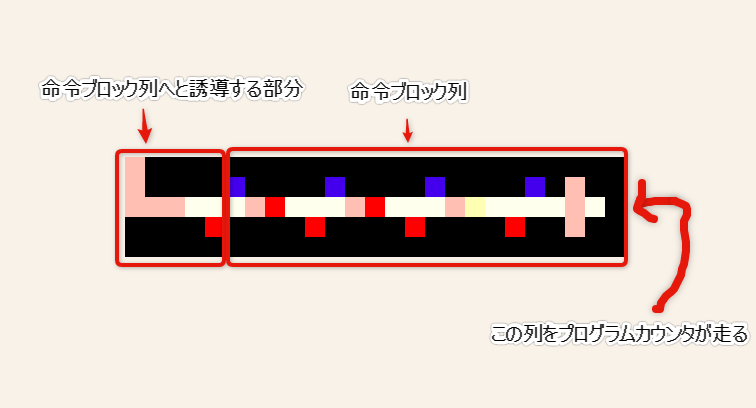
\includegraphics[width=\textwidth]{images/783f2ae98363220ed6859c9bd97cb4ff.png}} \\
赤と青のポッチは接続方向を表すマーカなので、
本質的には不要なので無視してください。

一直線のブロックの列だと、分岐もループもできず、
つまり構造化定理の順次しか実現できないので、
殆どのプログラムを書くことは出来ません。
が、この時点でHello Worldは書けますね。

で、次は分岐を作るわけですが、 Pointerという良い命令がPietにはあって、
それを使うとDP、つまり進む向きを変えられます。 Notという命令もあって、
それを使うとスタックの先頭が0の時だけ先頭を1に変え、
それ以外の時は先頭を0に変えられます。
Pointer命令はスタックのトップの値を見て、
その数だけDPを時計回りに回します。
これを使えば、スタックの先頭が0の時に分岐するようなものが作れます。

\url{https://gyazo.com/3c7bc0cb0dd41680c6b652ef4486b390}\\
\href{https://gyazo.com/3c7bc0cb0dd41680c6b652ef4486b390}{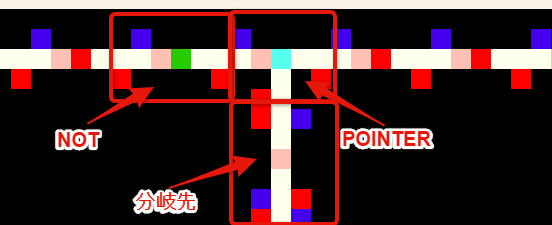
\includegraphics[width=\textwidth]{images/3c7bc0cb0dd41680c6b652ef4486b390.png}} \\
スタックの先頭が0以外の時はそのまま直進し、
0の時は下に分岐します。

これで分岐することには成功したので、
適当なところに合流したいと思います。

\url{https://gyazo.com/4f893a8b1a52e2de3f9bd70338ebb9b8}\\
\href{https://gyazo.com/4f893a8b1a52e2de3f9bd70338ebb9b8}{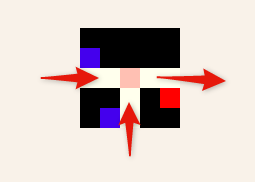
\includegraphics{images/4f893a8b1a52e2de3f9bd70338ebb9b8.png}} \\
このような構造でプログラムカウンタが下から来た場合と左から来た場合に合流してともに右に流すことができるので、
ここに飛んで来るジャンプのようなものが書けて、
あとはすぐにわかる構造で、以下の様な後ろ向きへの条件付きジャンプができます。

\url{https://gyazo.com/846e9f87a072a65e02e6943e20adc534}\\
\href{https://gyazo.com/846e9f87a072a65e02e6943e20adc534}{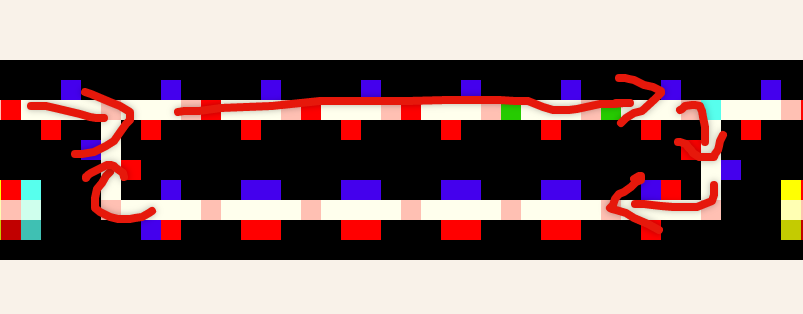
\includegraphics[width=\textwidth]{images/846e9f87a072a65e02e6943e20adc534.png}}

これとよく似た感じで、少し考えれば以下のように前向きに条件付きジャンプができます。

\url{https://gyazo.com/83ac7efa68410f18a8cfdfa1ba52d2ee}\\
\href{https://gyazo.com/83ac7efa68410f18a8cfdfa1ba52d2ee}{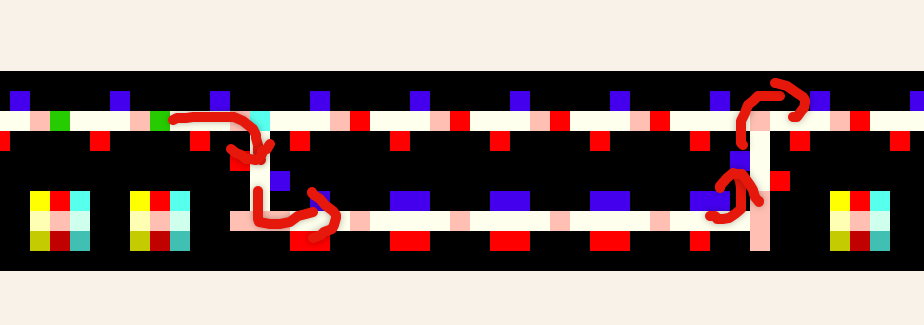
\includegraphics[width=\textwidth]{images/83ac7efa68410f18a8cfdfa1ba52d2ee.png}}

ここまでくれば、後は必要な物を幾つか用意するだけでどんなプログラムだって書くことが可能です。

ここまでやってきたようなものを使い、javascriptでCanvasの上にベタベタとブロックを重ねてゆきます。
ブロックは心をこめて手でPidetを使い打ちます。

生成されるコードの例を幾つか上げます。

数字を1つ入力として取り、それが奇数なら1、偶数なら0を出力するPietです。
Piet-automataでは、以下の様な擬似コードを書いて、それをPietへと変換します。
命令の詳細は\url{https://github.com/nna774/piet-automata/blob/master/README.md}にあるので、
そちらを参照してください。
\url{https://github.com/nna774/piet-automata/blob/master/tests/even-or-odd.pas}
\begin{lstlisting}[frame=single]
INN
PUSH 1
DUP
ADD
MOD
JEZ zero
PUSH 1
OUTN
HALT
LABEL zero
PUSH 1
NOT
OUTN
HALT
\end{lstlisting}
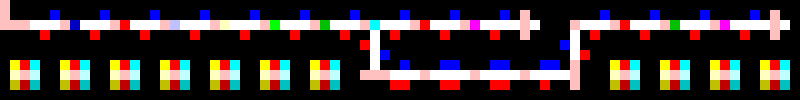
\includegraphics[width=\textwidth]{images/bb3413d9656b9449ffa280423c769389.png}


2つ数字を入力として取り、GCDを出すPietです。Cで言うと
\begin{lstlisting}[frame=single, language={C}]
int gcd(int n, int m) {
  int tmp;
  if (n < m) return gcd(m, n);
  tmp = n % m;
  if (tmp == 0) return m;
  return gcd(m, tmp);
}
main() {
  int n, m;
  scanf("%d", &n); scanf("%d", &m);
  printf("%d", gcd(n, m));
}
\end{lstlisting}
のようなことをしています。
\url{https://github.com/nna774/piet-automata/blob/master/tests/gcd.pas}
\begin{lstlisting}[frame=single, language=]
INN
DUP
INN
DUP
PUSH 3
PUSH 1
ROLL
GREATER
JEZ S
PUSH 2
PUSH 1
ROLL
LABEL S
# ここでスタックに二つ入っていて、大きいほうが上
PUSH 2
PUSH 1
ROLL
DUP
PUSH 3
PUSH 1
ROLL
# 小さい方は使うのでコピー
MOD
DUP
JEZ END
PUSH 2
PUSH 1
ROLL
JMP S
LABEL END
POP
OUTN
\end{lstlisting}

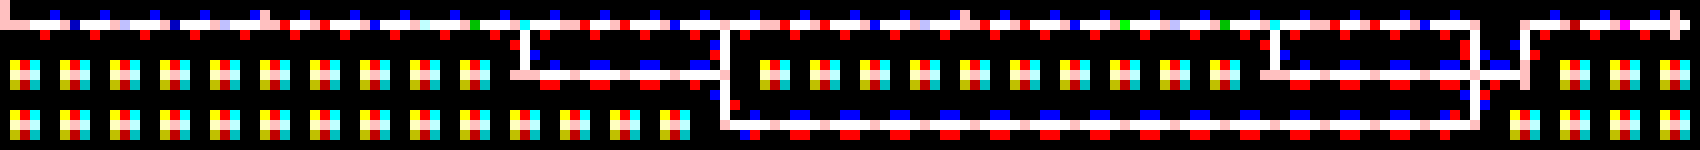
\includegraphics[width=\textwidth]{images/6c82e735b7bd782e1f328f3d309c1286.png}

実は最新のpiet-automataではブロックのサイズを3x3にすることに成功しているので、
以下のようになります(ここまでは説明するときにわかりやすいかと思い5x5のブロックばかり出してきました)。

奇遇判定\\
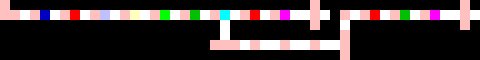
\includegraphics[width=\textwidth]{images/e3bbb6f046fe9aa8d7c0ae5d01e34798.png}

GCD\\
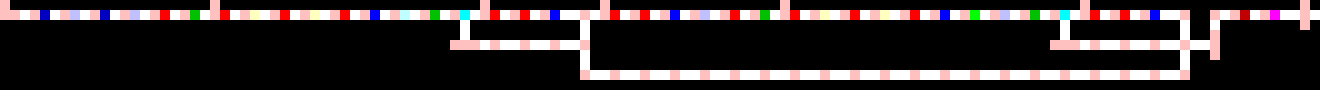
\includegraphics[width=\textwidth]{images/4a63cd9654933cc75ca74e60f3982241.png}

\section{おわりに}

とまぁだいたいこんな感じでPietの擬似命令の列からPietの画像を生成しています。
今回はだいぶ実装の詳細は省いたので、
詳細が知りたい方は\url{https://github.com/nna774/piet-automata}をご覧ください。
今回書いたことをだいたいそのまま実装して、
幾つかの最適化をかけたような感じです。
`/piet' の中にブロックが入っていて、`config.js'にその対応が入っています。

もう少し高級な言語から擬似命令列を生成できるようなものを作りたいと考えてはいるのですが、
まだ実装はありません。

最後に幾つかこのレポジトリに関連したものを友人が作ってくれたので、
紹介しておきます。

\begin{itemize}
\item
  \url{https://github.com/primenumber/pasxx} 私の擬似命令に拡張命令を追加して、
  piet-automataで使える列に変換できるものです。
  サイズが巨大になりがちなので少し厳しいです。
\item
  \url{https://github.com/1995hnagamin/pas-interpreter} 擬似命令列をPietに落とさずにそのまま実行できるスクリプトです。
\end{itemize}

今回初挑戦の拙い文章でしたが、ここまで読んでくださってありがとうございました。


\chapter{僕の考えた最強のPiet拡張}

\section{はじめに}

murataと申します.TwitterIDは@paradigm\_9です.
nona7さんと同じくKMC(京大マイコンクラブ)というサークルに所属しています.
今回Pietで一つのサークルとして出店するという@nona7さんの挑戦を聞いて,
「これは寄稿するしかない!」と勢いだけで寄稿します.
僕は強いプログラミングが書けないので,お絵かき的なPietを描いて楽しんでいます.

\section{Pietは凄い!}

今現在様々な言語が世の中にはありますが,
Pietは画像でプログラミングが出来るというとても異彩な言語です.
画像でプログラミングが出来るというのは大変すごいことです.
例えば,一見キャラクターの顔画像にしか見えないのに,
Pietとして実行すると「72CHIHAYA」と出力し続けるものを描いたことがあります.\\\includegraphics{images/0c1bff41d6d4f3358e682af6f3c112c4.png}

rubyが「プログラミングが楽しく出来るように」を, perlが「There's more
than one way to do it(やり方は一つじゃない)」を モットーにしていますが,
Pietは画像でプログラミングが出来るので楽しく,
上記の例のようにプログラミングを表現する絵は自分の好きなように描けますので,
PietはRubyやPerlとおなじコンセプトを持った凄い言語と言えるでしょう!

\section{僕の考えた最強のPiet (Piet\#)}

そんな素晴らしいPietですが,未だに難解プログラミング言語として扱われています.
Piet自体には本当はもっと表現力があるのに\ldots{}.
今回の記事は,そんなPietを拡張してもっともっと実用的な
最強のPiet「Piet\#」の仕様を考えたという記事です.

\section{Piet\#の新機能}

\begin{itemize}
\item
  DLLのインポート
\item
  他のPietのコードの呼び出し
\item
  スタックにスタックを積める
\item
  強力な文字処理機構
\item
  自分の好きな18色によるコーディング
\end{itemize}

\section{Piet\#で新たに出来ること}

\subsection{Webアプリケーションやゲームを簡単に作れる!}

旧Pietでは標準入出力になにかをするので手一杯でした.
しかし,Piet\#では前述のDLLのインポートをサポートしているので,
気軽に素晴らしいプログラミングができます!
更に,他のPietコードを呼び出せるので,
作成した機能はモジュール化することができ,
ライブラリを揃えれば上述のことはたやすく実現できます!

\subsection{高い表現力により自由なコーディングが出来る!}

旧Pietでは数字しかスタックに積めませんでした.
そのため,とても表現力が低かったのです.
しかし,Piet\#では,新たにスタックにスタックを積むことが出来て,
とても表現力豊かなプログラミングが出来ます.
スタックにスタックに,\ldots{},スタックに,スタックを積むというふうに
無限にスタックにはスタックを積めるので,
木構造のようなデータ構造も再現できます.
また,新たにスタックに積んだスタックを
文字列とみなすことで高度な文字処理が出来る機構も搭載していて,
ファイル処理や高度な文字処理にも耐えうるコーディングが可能となります.

\subsection{楽しく直感的なプログラミングが出来る!}

旧Pietでも楽しくプログラミングが出来たのですが,
コメントの挿入も出来ず,決まった18色しか出来ないなどの成約がありました.
しかし,Piet\#では専用のIDEでそれらをカバーする予定です.
また,Piet\#のプログラミングで本質的に変わったことは,
新たにスタックが積めるようになったことだけなので,
学習コストも少なくて済みます!
Pietがコードとして利用するPNG画像にはメタデータを挿入できることを利用して,
コメントの挿入,好きな18色でのコーディングなどをサポートし,
より快適なプログラミングを目指します!

\section{PietとしてのPiet\#}

Piet\#はあくまでもPietです. 色は18色しか扱わないし,
画像のみがあれば誰でも同じコードを再現できます.
これらを守ることで,Cに対するC++のように,
旧Pietのコードもそのまま動かすことが可能となります.

\section{色の問題}

Piet標準色はチカチカするものばかり\ldots{}
しかも特に青系の色など,違いがわかりにくいものもあります.
Piet\#では,自分で18色を定義できます.
とはいえ,好き勝手定義しては読みにくいですので,指針を.
色相(H)の順序付けが出来て,明度(彩度)の順序付けができればいいですよね.
6色なので,色相は基本的には60度程度違えばよいですね.
色を見分けられるように,30度以上の差を全てが保つ色にしましょう.
明度と彩度でSVの三角形は,色が分かるように, 0.5 \textless{} V \textless{}
1 ,0.2 \textless{} S \textless{}= 1であるという条件のもと,
V,Sを変えればすきな組み合わせに出来ますね.

\section{Piet\#としての情報の保存方法}

Piet\#(Pietも!)が実行するコードはPNGファイルです.
実はPNGにはメタデータを入れることが出来ます.
Piet\#のIDEではコメントを挿入することが出来ます.
また,前述のとおり18色の指定も出来ます.
そのほかにも,IDEとして保存しておきたい情報は数多くあります.
それも全てこのメタデータに保存すればよいですね.

\section{記法の定義}

今までの項でPiet\#の新たな機能を見ました.
以降の項でPiet\#の具体的な仕様を見ていくことにしましょう.
まずは記法の定義から見ていきましょう. DirectionPointerをDPと略します.
CodelChooserをCCと略します.

空のスタックに順番に, \textbf{1 をPush, 2 をPush, 3 をPush, 4 をPush}
した時, スタックの変化を \textbf{{[}{]} $\to$ {[}1{]}
$\to$ {[}1,2{]} $\to$ {[}1,2,3{]} $\to$
{[}1,2,3,4{]}} と表記します.
つまり,一番右にあるものが一番最近Pushしたものとなります.

また, \textbf{{[}1,2,3,4{]}} にAdd命令を行うことを, \textbf{Add
{[}1,2,3,4{]} $\to$ {[}1,2,7{]}} と表記できます. この場合,1,2
は直接演算に関係ないので, \textbf{Add {[}\ldots{},3,4{]} $\to$
{[}\ldots{},7{]}} のように記すことができます. さらに演算に関係ない項目
\textbf{\ldots{}} を省略し,以降の文章では \textbf{Add {[}3,4{]}
$\to$ {[}7{]}} のように記します. 例えば,Sub{[}7,2{]}
$\to$ {[}5{]} は,7 - 2 = 5 をしたことを意味しますね.

また,Piet\#では前述のとおり数字とスタックのみで構成されています.
しかし,文字処理のために糖衣構文を定義しておきます. まず,65 =``A''; 66
=``B'';67 =``C'';とUnicodeで対応しています. 文字処理のために
{[}65,66,67{]} と積んだ場合,
その数字が何を指しているかで表現したほうが見やすいので, {[}65,66,67{]} =
{[}A,B,C{]} と表記しましょう. さらにもっと省略して,{[}A,B,C{]} = ``ABC''
という糖衣構文も定義します. Piet\#
では数字とスタックしか使わないということは
大事なことなので忘れないでください.  

\section{モジュール呼び出しとスタック型の導入}

Piet\#では新たに2つの命令を導入します.
既存のPietと競合しないように導入しなければなりません.
そこで,普通しない命令である 0除算命令,0剰余命令に
新たな命令としての意味を持たせるという形で導入します.

\paragraph{モジュール呼び出し}

\textbf{Div {[}n,0{]} $\to$ {[}{]}}\\\textbf{n.png
という名前のPietを読み込んで実行します.}\\現在の標準入力,標準出力,スタックのまま,
そしてDP は 0 ,CC は 1 で初期化されて
そのPietを一番左上の位置から実行します.
終了後,退避されていたDP,CCは元に戻ります.
この命令によりファイルをモジュール化でき,
ファイルの分割が可能になります.
また,言語としての強さの要素である標準ライブラリを搭載し
簡単にこの命令でアクセス出来るように,
nが負の場合は標準ライブラリから探すというふうにする予定です.

\paragraph{スタックの新規作成}

\textbf{Mod {[}\ldots{},x1,x2,\ldots{},xn,n,0{]} $\to$
{[}\ldots{},{[}x1,x2,\ldots{},xn{]}{]}}\\\textbf{深さnまでの要素を積んだ新たなスタックをPushします}\\この関数により,Piet\#のスタックに,
新たなスタックを積むことが出来るようになります\\例: Mod
{[}\ldots{},C,H,Y,3,0{]} $\to$ {[}\ldots{},{[}C,H,Y{]}{]}

\section{スタック演算}

今回の拡張によって数字だけでなくスタックも積めるようになりました.
スタック同士の演算を新たに定義しましょう.
スタックとスタック,数字と数字との演算なら問題はないのですが,
スタックと数字が混じっていた場合についてはちょっと考えないといけません.
結論としては,その数字を一つのみを積んだ新たなスタックを作成して,
それを利用してスタックとスタックの演算として扱います.

例えば,加算の関数 Add は, \textbf{Add {[}\ldots{},72,28{]}
$\to$ {[}\ldots{},100{]}} と,数字同士なら演算されますが,
スタック同士に Add を作用させると結合の意味になります.\\例:) \textbf{Add
{[}\ldots{},{[}A,B,C{]},{[}X,Y{]}{]} $\to$
{[}\ldots{},{[}A,B,C,X,Y{]}{]}}\\そして,数字とスタックの演算の場合は,
その数字を一つのみを積んだ新たなスタックを作成して,
それを利用してスタックとスタックの演算として扱うので, \textbf{Add
{[}\ldots{},C,{[}H,Y{]}{]} $\to$ Add
{[}\ldots{},{[}C{]},{[}H,Y{]}{]} $\to$
{[}\ldots{},{[}C,H,Y{]}{]}} と計算されます.

それでは早速命令を見ていきましょう!

\subsection{ゼロ引数関数}

Push , In(char) , In (number) はスタックとしては定義されません.

\subsection{一引数関数}

スタックの先頭から一つとり,それに演算を適用します.

\paragraph{Switch: 平坦化する (Flatten)}

型 :: {[}\ldots{}{]} $\to$
{[}\ldots{}{]}\\スタックにスタックが積まれて,更にそれにスタックが\ldots{}という状態に
陥いったときにそれを全て平坦化してくれます. 例を見てみますよ.

\begin{itemize}
\item
  Switch {[}\ldots{},{[}A,{[}B,C,{[}D{]},E{]},F,G{]}{]} $\to$
  {[}\ldots{},{[}A,B,C,D,E,F,G{]}{]}
\item
  Switch {[}\ldots{},{[}A,B,C{]}{]} $\to$
  {[}\ldots{},{[}A,B,C{]}{]}
\item
  Switch {[}\ldots{},{[}A{]}{]} $\to$ {[}\ldots{},{[}A{]}{]}
\item
  Switch {[}\ldots{},{[}{]}{]} $\to$ {[}\ldots{},{[}{]}{]}
\end{itemize}

\paragraph{Point : スタックの先頭を取得する}

型 :: {[}\ldots{},T{]} $\to$ {[}\ldots{}{]},
T\\スタックの先頭要素を一つとりだしてPushします.例をあげましょう.

\begin{itemize}
\item
  Point {[}\ldots{},{[}A,B,C{]}{]} $\to$
  {[}\ldots{},{[}A,B{]},C{]}
\item
  Point {[}\ldots{},{[}A,B,C,{[}X,Y{]}{]}{]} $\to$
  {[}\ldots{},{[}A,B,C{]},{[}X,Y{]}{]}
\item
  Point {[}{[}{[}Xn,Yn{]},\ldots{},{[}X1,Y1{]}{]}{]} $\to$
  {[}{[}{[}Xn,Yn{]},\ldots{},{[}X2,Y2{]}{]},{[}X1,Y1{]}{]}
\item
  Point {[}\ldots{},{[}A{]}{]} $\to$ {[}\ldots{},{[}{]},A{]}
\item
  Point {[}{[}{]}{]} $\to$ {[}{]}
\end{itemize}

\paragraph{Dup: コピーする (Duplicate)}

型 :: {[}\ldots{}{]} $\to$ {[}\ldots{}{]},{[}\ldots{}{]}
数字版のDupと同じです.例を見せます.

\begin{itemize}
\item
  Dup {[}\ldots{},{[}{[}1,3,4{]},4,32{]}{]} $\to$
  {[}\ldots{},{[}{[}1,3,4{]},4,32{]},{[}{[}1,3,4{]},4,32{]}{]}
\end{itemize}

\paragraph{Not: スタックの中身が空の時 1 を,それ以外では 0 を返す}

型 :: {[}\ldots{}{]} $\to$
Num\\数字版のNotと意味的には一緒です.
NotとSwitchを組み合わせることで条件分岐に使用出来ますね.

\begin{itemize}
\item
  Not {[}``Hello''{]} $\to$ {[}0{]}
\item
  Not {[}{[}A{]}{]} $\to$ {[}0{]}
\item
  Not {[}{[}{]}{]} $\to$ {[}1{]}
\end{itemize}

\paragraph{Pop: 捨てる}

型 :: {[}\ldots{}{]} $\to$
{[}{]}\\数字版のPopと一緒です.例を一応載せときます.

\begin{itemize}
\item
  Pop {[}{[}A,B,C{]}{]} $\to$ {[}{]}
\end{itemize}

\paragraph{Out(Char) : 文字列として出力する}

型 :: {[}\ldots{}{]} $\to$ {[}{]}\\
Switchで平坦化して文字列と見なせるようにしてから出力します.

\begin{itemize}
\item
  Out(Char) {[}{[}C,H,Y{]}{]} $\to$ {[}{]} : ``CHY''と出力する
\item
  Out(Char) {[}{[}千,早{]}{]} $\to$ {[}{]} :
  ``千早''と出力する
\item
  Out(Char) {[}{[}C,{[}H,I,{[}H,A{]},Y{]},A{]}{]} $\to$ {[}{]}
  : ``CHIHAYA''と出力する
\item
  Out(Char) {[}{[}C{]}{]} $\to$ {[}{]} : ``C'' と出力する.
\item
  Out(Char) {[}{[}{]}{]} $\to$ {[}{]} : 何も出力しない.
\end{itemize}

\paragraph{Out(Num) : スタックの中身を全て取り出し,先頭に要素数を積む}

型 :: {[}Tn,\ldots{},T1{]} $\to$ Tn,\ldots{},T1,Num\\Out(Num)
という名前ですが出力はしませんので注意して下さい.
Mod0命令の逆演算となります.

\begin{itemize}
\item
  Out(Num) {[}\ldots{},{[}A,B,C{]}{]} $\to$
  {[}\ldots{},A,B,C,3{]}
\item
  Out(Num) {[}\ldots{},{[}A,{[}B,C{]},D{]}{]} $\to$
  {[}\ldots{},A,{[}B,C{]},D,3{]}
\item
  Out(Num) {[}\ldots{},{[}A{]}{]} $\to$ {[}\ldots{},A,1{]}
\item
  Out(Num) {[}\ldots{},{[}{]}{]} $\to$ {[}\ldots{},0{]}
\end{itemize}

\paragraph{Div 0: モジュール呼び出し}

Div 0 の 被除数が スタックの場合,それをSwitchで平坦化して
文字列にし,その文字列のパスにあるPietモジュールを実行します.

\paragraph{Mod 0 : スタックの新規作成}

Mod {[}\ldots{},x1,x2,\ldots{},xn,n,0{]} $\to$
{[}\ldots{},{[}x1,x2,\ldots{},xn{]}{]}\\深さnまでの要素を積んだ新たなスタックをPushします.
x1,\ldots{},xn がスタック型であっても大丈夫です. n
がスタックであった場合は n = ∞ として(つまり深さ無限で)演算します.

\begin{itemize}
\item
  Mod {[}\ldots{},C,H,Y,3,0{]} $\to$
  {[}\ldots{},{[}C,H,Y{]}{]}
\item
  Mod {[}\ldots{},{[}C,H,I{]},{[}H,A,Y,A{]},2,0{]} $\to$
  {[}\ldots{},{[}{[}C,H,I{]},{[}H,A,Y,A{]}{]} {]}
\item
  Mod {[}\ldots{},C,H,Y,{[}{]},0{]} $\to$
  {[}{[}\ldots{},C,H,Y{]}{]}
\end{itemize}

\subsection{二引数関数}

スタックの先頭から2つとり,それらに演算を適用します.

\paragraph{Add: 結合する (Append)}

型 :: {[}\ldots{}{]},{[}\ldots{}{]} $\to$
{[}\ldots{}{]}\\単純に結合します.例を示します. {[}A,B,C{]} =``ABC''
という糖衣構文を思い出してくださいね.

\begin{itemize}
\item
  Add {[}\ldots{},{[}C,H,I{]},{[}h,a,y,a{]}{]} $\to$
  {[}\ldots{},{[}C,H,I,h,a,y,a{]}{]}
\item
  Add {[}\ldots{},``CHIhaya'',``isGOD'') $\to$
  {[}\ldots{},``CHIhayaisGOD''{]}
\item
  Add {[}\ldots{},1,{[}10,100,1000{]}{]} $\to$
  {[}\ldots{},{[}1,10,100,1000{]}{]}
\item
  Add {[}\ldots{},{[}1,10,100{]},1000{]} $\to$
  {[}\ldots{},{[}1,10,100,1000{]}{]}
\item
  Add {[}\ldots{},{[}A,B,C{]},{[}{]}{]} $\to$
  {[}\ldots{},{[}A,B,C{]}{]}
\item
  Add {[}\ldots{},{[}{]},{[}{]}{]} $\to$ {[}\ldots{},{[}{]}{]}
\end{itemize}

\paragraph{Sub: 正規表現で分割する (Split)}

型 :: {[}\ldots{}{]},{[}\ldots{}{]} $\to$
{[}\ldots{}{]}\\Switch
で平坦化し,文字列として見なせるようにしてからSplitします. {[}A,B,C{]}
=``ABC'' という糖衣構文を思い出してくださいね.

\begin{itemize}
\item
  Sub {[}\ldots{},``Pietはx楽しい'',``x''{]}$\to$
  {[}\ldots{},{[}``Pietは'',``楽しい''{]}{]}
\item
  Sub {[}``12/12 21:41''," \textbar{}/\textbar{}:``{]} $\to$
  {[}{[}''12``,''12``,''21``,''41"{]}{]}
\item
  Sub {[}\ldots{},``helloHWWH!'',H{]} $\to$
  {[}\ldots{},{[}``hello'',{[}W,W{]},{[}!{]}{]}{]}
\item
  Sub {[}\ldots{},{[}h,{[}e,H{]},{[}l,l,{[}{[}o{]}{]}{]}{]},{[}H{]}
  $\to$ {[}\ldots{},{[}``he'',``llo''{]}{]}
\item
  Sub {[}\ldots{},H,``\\s''{]} $\to$ {[}\ldots{},{[}H{]}{]}
\item
  Sub {[}\ldots{},H,``H''{]} $\to$ {[}\ldots{},{[}{]}{]}
\end{itemize}

\paragraph{Mul: 直積集合を取得する}

型 :: {[}\ldots{}{]},{[}\ldots{}{]} $\to$
{[}\ldots{}{]}\\便利な未来を作る直積集合ですよ.

\begin{itemize}
\item
  Mul {[} {[}A,B,C{]},{[}X,Y{]} {]} $\to$ {[}
  {[}{[}A,X{]},{[}A,Y{]},{[}B,X{]},{[}B,Y{]},{[}C,X{]},{[}C,Y{]}{]} {]}
\item
  Mul {[}\ldots{},H,{[}J,I{]}{]} $\to$ {[}\ldots{}, {[}
  {[}H,J{]},{[}H,I{]} {]} {]}
\item
  Mul {[}\ldots{},{[}A{]},H{]} $\to$ {[}\ldots{},{[}A,H{]}{]}
\item
  Mul {[}\ldots{},{[}{]},A{]}$\to$ {[}\ldots{},{[}{]}{]}
\item
  Mul {[}{[}A,B,C{]},{[}{[}X,Y{]}{]}{]} $\to$
  {[}{[}A,{[}X,Y{]}{]},{[}B,{[}X,Y{]}{]},{[}C,{[}X,Y{]}{]}{]}
\item
  これにより,例えば 0 \textless{} n,m $\leq$ 20 の n * m
  の取りうる値を列挙できます
\end{itemize}

\begin{itemize}
\item
  1〜20までと20と0を順に積む $\to$ {[}1,\ldots{},20,20,0{]}
\item
  Mod0 を実行してスタック化 $\to$ {[}{[}1,\ldots{},20{]}{]}
\item
  Dupでコピーを作成 $\to$
  {[}{[}1,\ldots{},20{]},{[}1,\ldots{}20{]}{]}
\item
  Mul で直積を取る $\to$
  {[}{[}{[}1,1{]},\ldots{},{[}20,20{]}{]}{]}
\item
  Point で先頭の要素を取得 $\to$
  {[}{[}{[}1,1{]},\ldots{},{[}20,19{]}{]},{[}20,20{]}{]}
\item
  Out(N)で分解する $\to$
  {[}{[}{[}1,1{]},\ldots{},{[}20,19{]}{]},20,20,2{]}
\item
  2 を Pop $\to$
  {[}{[}{[}1,1{]},\ldots{},{[}20,19{]}{]},20,20{]}
\item
  Mulで掛け算する $\to$
  {[}{[}{[}1,1{]},\ldots{},{[}20,19{]}{]},400{]}
\item
  Roll 2 1 で入れ替える $\to$
  {[}400,{[}{[}1,1{]},\ldots{},{[}20,19{]}{]}{]}
\item
  5\textasciitilde{}9 を繰り返す.
\item
  {[}400,\ldots{},1{]} が出来上がる.
\end{itemize}

\paragraph{Div: 正規表現でマッチさせる (Match)}

型 :: {[}\ldots{}{]},{[}\ldots{}{]} $\to$
{[}\ldots{}{]}\\Switch
で平坦化し,文字列として見なせるようにしてからMatchします. {[}A,B,C{]}
=``ABC'' という糖衣構文を思い出してくださいね.

\begin{itemize}
\item
  Div {[}``aa9bb1cc'',``.{[}1-9{]}.''{]} $\to$
  {[}{[}``a9b'',``b1c'',``aa9bb1cc''{]}{]}
\item
  Div {[}``aa'',``.{[}1-9{]}.''{]} $\to$ {[}{[}{]}{]}
\item
  Div {[}``aHxH'',H{]}$\to$ {[}{[}``H'',``H'',``aHxH''{]}{]}
\item
  Div {[}H,``h\textbar{}H''{]} $\to$ {[}{[}``H'',``H''{]}{]}
\item
  Div {[}{[}{]},``A\textbar{}B''{]} $\to$ {[}{[}{]}{]}
\item
  Div {[}``ABC'',{[}{]}{]} $\to$ {[}{[}{]}{]}
\end{itemize}

\paragraph{Mod: スタックを順番に結合する (Combine)}

型 :: {[}\ldots{}{]},{[}\ldots{}{]} $\to$
{[}\ldots{}{]}\\それぞれの要素を結合します。Mulと上手く組み合わせてご使用下さい。

\begin{itemize}
\item
  Mod {[}``01234'',``abc''{]} $\to$
  {[}{[}``2a'',``3b'',``4c''{]}{]}
\item
  Mod {[}{[}a,b,c,d,e{]},{[}x,y{]}{]} $\to$
  {[}{[}{[}d,x{]},{[}e,y{]}{]}{]}
\item
  Mod {[}{[}{[}a,b,c{]},{[}d,e{]}{]},{[}x,y{]}{]} $\to$
  {[}{[}{[}{[}a,b,c{]},x{]},{[}{[}d,e{]},y{]}{]}{]}
\item
  Mod {[}H,``abc''{]}$\to$ {[}{[}H,c{]}{]}
\item
  Mod {[}``abc'',H{]}$\to$ {[}{[}c,H{]}{]}
\item
  Mod {[}``abc'',{[}{]}{]}$\to$ {[}{[}{]}{]}
\item
  Mod {[}{[}{]},{[}{]}{]}$\to$ {[}{[}{]}{]}
\end{itemize}

\paragraph{Greater: ファイルを読み書きする}

型 :: {[}\ldots{}{]},{[}\ldots{}{]} $\to$
Num\\ファイルを開いて標準入出力へリダイレクトします. 成功したら 1
,失敗したら 0 が積まれます. 第一引数は開くファイル名です.
第二引数は開くモードを指定します.\\\textbf{モード}

\begin{itemize}
\item
  {[}R{]} or {[}r{]} or {[}0{]} : 読み込み(Read)モードで開く.
\item
  {[}W{]} or {[}w{]} or {[}1{]} : 書き込み(Write)モードで開く.
\item
  {[}A{]} or {[}a{]} or {[}2{]} : 追加書き込み(Append)モードで開く
\item
  {[}CR{]} or {[}cr{]} or {[}3{]} : Readで開いたファイルを閉じる.
\item
  {[}Cw{]} or {[}cw{]} or {[}4{]} : Writeで開いたファイルを閉じる.
\item
  その他 : 現在開いているファイルをRead,Writeともに閉じる.
\end{itemize}

新たにファイルを開いた場合,現在開いているファイルは閉じられます.
例を示します.

\begin{itemize}
\item
  Greater {[}``f1.txt'',r{]} $\to$ {[}1{]} :
  f1.txtを開き標準入力をリダイレクトする
\item
  Greater {[}``f2.txt'',1{]} $\to$ {[}1{]} :
  f2.txtを開き標準出力をリダイレクトする
\item
  Greater {[}``f.t'',r{]} $\to$ {[}0{]} : f.tが開けなかった.
\item
  \begin{description}
  \item[Greater {[}``f3.txt'',a{]} $\to$ {[}1{]}]
  2.で開いていたf2.txtを閉じて新たにf3.txtを
  \end{description}

  追加書き込みモードで開き,標準出力をリダイレクトする.
\item
  Greater {[}{[}{]},{[}cr{]}{]} $\to$ {[}0{]} :
  1.で開いていたf1.txtを閉じる.
\end{itemize}

\subsection{四引数関数}

\subsection{Roll: Dllを読み込む}

型 :: {[}\ldots{}{]},{[}\ldots{}{]},{[}\ldots{}{]},{[}\ldots{}{]}
$\to$ Num or {[}\ldots{}{]} or
Empty\\Pietが何でも出来るようになる魔法の関数です.
この関数により,ゲームやアプリを作ることが出来るようになります.
実用的なマルチメディアな操作をPietで体感しよう!\\\textbf{引数}\\第一引数
: DLLへのファイル名を含むパス\\第二引数 : DLL内の関数名\\第三引数 :
DLLに渡される型の宣言\\第四引数 :
DLLを呼び出すための引数リスト\\\textbf{例}

\begin{itemize}
\item
  Roll {[}``user32.dll'',``MessageBoxA'', ``vssui'', {[}{[}{]},``Hello
  World.'',``Caption'',0{]}{]}\\C製Dllであるuser32.dllの,MessageBoxA関数を呼び出します.
  ``vssui''というのは的確にDLLを扱う為の型情報の宣言です.
  引数の型は前から順に void*(HANDLE),char(LPSTR),
  char*(LPSTR),unsigned int (UINT) で,
  返り値はint型にするという宣言で,
  前から順にvoid*,char*,char*,unsigned int,intなので 頭文字をとって
  ``vssui''です.
\item
  Roll
  {[}``TestDLL.dll'',``TestDll.CsDll.LangA'',0,{[}123,``RA''{]}{]}\\自作.Net製DllでTestDll.CsDll.LangA(123,``RA'')を実行します.
  第二引数は NAMESPACE.CLASSNAME.STATICFUNCTIONNAME とします.
  .Net製Dllは型情報が内蔵されているために,
  型を推論することができ,第三引数は省略できます.
   というか,型を書いても無視されます.
  C製Dllで扱えるプリミティブな型以外はサポートしません.
\end{itemize}

\subparagraph{DLL読み込みの型}

Pietの最強のIDEであるPidetがC\#製なので
Piet\#のIDE,実行ファイルもC\#製です. そのため,内部的にはC\#で処理します.
型の相互変換表は下のようになります.

\begin{table}[htb]
    \begin{tabular}{llll}
      Pietでの型 & Cでの型 & Cでの別名 & C\#での型 \\ \hline \hline
      Number & int,long & INT,LONG,BOOL & int \\
      Number & unsigned int,unsigned long & UINT,DWORD,ULONG & uint \\
      Number & unsigned char & BYTE & byte \\
      Number & char & CHAR &char \\
      Number & unsigned short & WORD &ushort \\
      Number & short & SHORT & short \\
      Number & float & FLOAT & float \\
      Stack & char* & LPSTR,LPWSTR & string \\
      Stack & void* & HANDLE & IntPtr
    \end{tabular}
\end{table}

\section{実装}

ここまで,仕様を詳細に示してきました. あとは実装するだけですね!
C\#で書かれたPidetがあるのでそれをforkして作りたいと思います. Piet\#.exe
を実行すれば出来るようにしたいですね.
スクリプト言語としてのPietとなって, Perl,PHP,Python,Piet\# の
4Pとなることを願っています.
このPiet\#プロジェクトは,ここまでの基本仕様が出来た時点で公開します.
オープンソースプロジェクトとして,
公開後は標準ライブラリの実装のContributeをお待ちしております! 最新情報は
Github : Muratam, Twitter : paradigm\_9 を参照下さい!


\chapter[あとがきの国]{あとがきの国}

\paragraph{NoNameA 774}

ここにはあとがきを書きます。

\paragraph{murata}

神はまずPietを作られた。世界は救われた。「ピエト福音書」より

\paragraph{PDF配布について}

今回値段の関係からカラーでの頒布を諦めたので(Pietは画像を扱うプログラムである以上、
ぜひカラーにしたかったのですが……)、
カラフルなPDFを配布させて頂きます。
以下のURIから、user:passはpiet:automataでダウンロードお願いします。
\url{https://nna774.net/piet/C89Book.pdf}



\null\vfill
\section*{奥付}
\hrule\vskip.5mm\hrule\vskip3mm
\begin{tabular}{ll}
  2015/12/31 & 初版発行\\
  hash: & \href{https://github.com/nna774/C89Book2/tree/3e0c955600ecae2e6549ea95b9c9eee7587ef01c}{3e0c955600ecae2e6549ea95b9c9eee7587ef01c}(の次)\\
  著作・発行 & NoNameA 774 (nonamea774@nnn77) \\
  サークル & いっと☆わーくす! \\
  メールアドレス & \href{mailto:nonamea774@gmail.com}{\nolinkurl{nonamea774@gmail.com}}\\
  Web & \url{https://nna774.net/}\\
  Twitter & @nonamea774\\
  GPG Key & 0x0C3E3AB2\\
  fingerprint & 674A 287A 21D2 2431 AD8F \\
  & D328 AEF3 C3C7 0C3E 3AB2
\end{tabular}
\vskip3mm\hrule\vskip3mm

表紙のPietはmurataによる"「ああ~心がぴょんぴょんするんじゃ~」と出力するチノちゃん"です。
\url{https://twitter.com/paradigm_9/status/677612736063258624}にて入手出来ます。


%% \newpage
%%  
%% \newpage
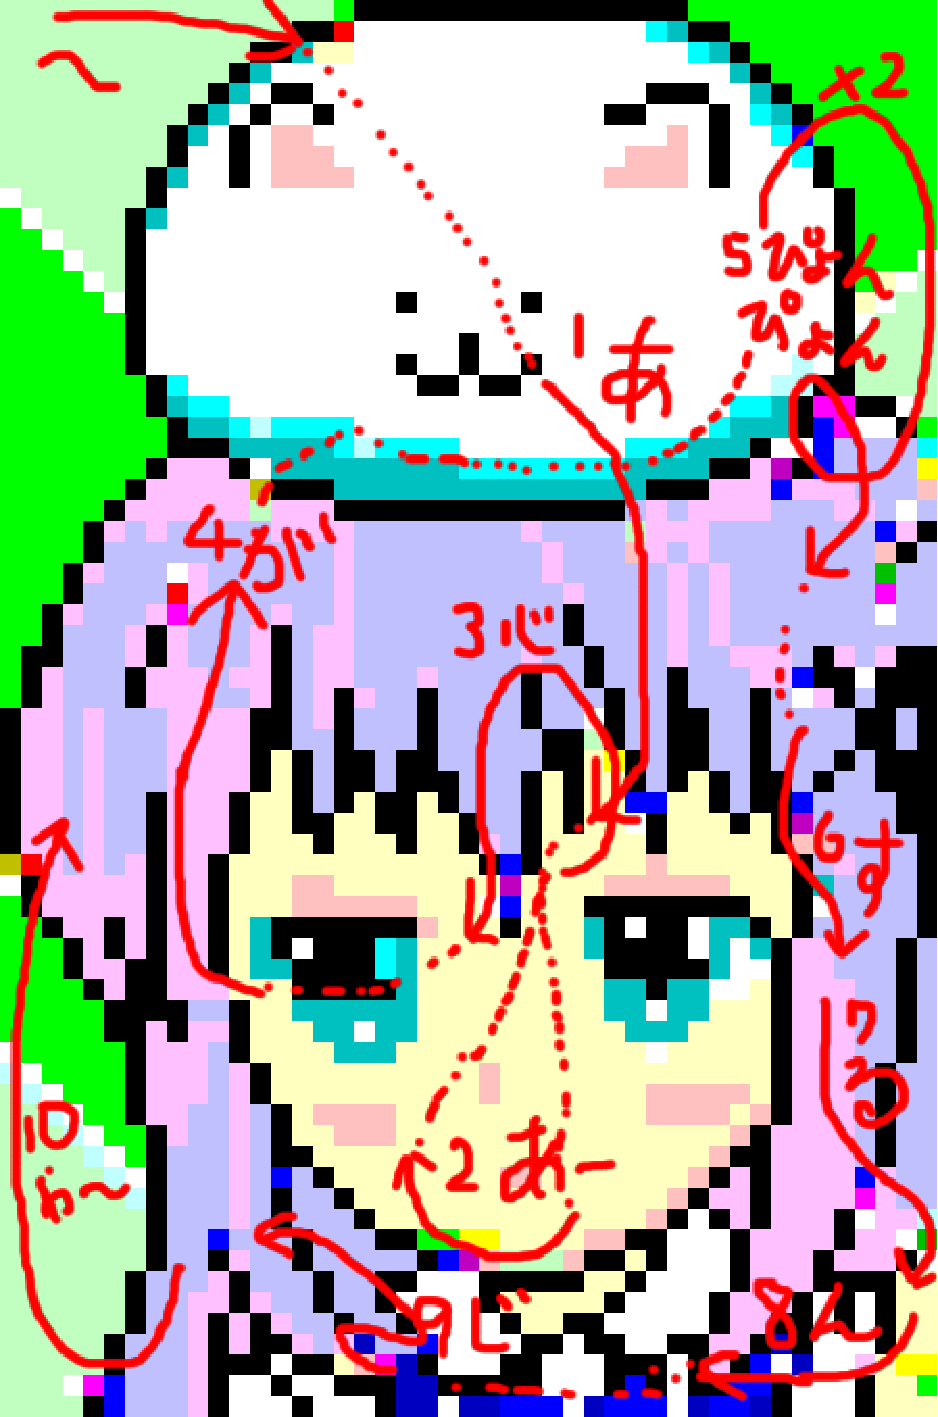
\includepdf{images/KOKORO100_kaisetsu.pdf}

\end{document}
